\documentclass[12pt]{article}

% Margins and spacing
\usepackage[margin=1in]{geometry}
\usepackage{setspace}
\onehalfspacing

% Packages
\usepackage{graphicx}
\usepackage{booktabs}
\usepackage{amsmath}
\usepackage{hyperref}
\usepackage{float}

\title{\textbf{BANA290 -- Assignment 4} \\
       \large AI Intensity and Firm Innovation: \\
       Instrumental Variable and Regression Discontinuity Analysis}
\author{Smart Campus Student App Incubator Archive \\
        Anteater Innovation Fund -- Spring Cohort}
\date{}

\begin{document}

\maketitle

% ============================================================
\section*{Interpretation of Results}
% ============================================================

\subsection*{IV vs Naive OLS Comparison}

The naive OLS regression estimates a positive and statistically
significant effect of AI intensity on innovation scores
(\textbf{+0.3245} points per compute hour, $p < 0.001$). However,
this estimate is biased upward because innovative teams naturally
invest more in AI -- creating a classic endogeneity problem where
ambition drives both AI usage and innovation scores simultaneously.

Using geographical distance to the campus fiber backbone as an
exogenous instrument, the 2SLS IV estimate falls to
\textbf{+0.1119} points per compute hour ($p = 0.403$). The OLS
overstates the true causal effect by nearly \textbf{three times}
relative to the IV estimate. The first-stage F-statistic of
\textbf{53.11} far exceeds the conventional threshold of 10,
confirming a strong and relevant instrument -- distance
meaningfully predicts AI intensity because closer teams benefit
from faster sync speeds and lower latency. The IV coefficient
is not statistically significant at conventional levels, likely
due to the limited sample size of 72 teams.

\subsection*{Exclusion Restriction}

Physical distance to the fiber node plausibly affects innovation
only through AI intensity access. There is no credible direct
channel from a team's dorm housing assignment to their innovation
score that bypasses compute usage. The instrument is geographically
determined and pre-assigned by the incubator, making it
effectively exogenous to team quality or ambition.

\subsection*{RDD Confirmation}

The RDD analysis at the 85-point eligibility cutoff strongly
confirms the direction of the IV findings. Teams just above the
threshold received server compute credits, enabling heavier AI
workloads and boosting innovation scores. The estimated
discontinuity jump is \textbf{+8.49 innovation points}
($p < 0.001$), a large and statistically significant effect.
The density plot shows no suspicious bunching of scores just
above 85, supporting the continuity assumption and ruling out
score manipulation. Figure~\ref{fig:plots} shows the RDD
scatter, first-stage relationship, and density check.

\subsection*{Policy Implications}

Both IV and RDD converge on the same conclusion: expanding
digital infrastructure access causally increases AI intensity
and, through it, innovation output. The strong first-stage
result ($F = 53.11$) shows that fiber proximity is a powerful
lever -- teams located closer to the engineering backbone
produce substantially more AI compute workloads. The RDD jump
of 8.49 points at the grant cutoff demonstrates that even
modest compute credit awards produce measurable innovation
gains at the margin. Policymakers and campus administrators
should prioritize fiber expansion into underserved housing
zones and lower eligibility thresholds for compute grant
programs to capture high-potential teams currently excluded
by arbitrary cutoffs.

% ============================================================
\section*{Figures and Tables}
% ============================================================

\begin{figure}[H]
    \centering
    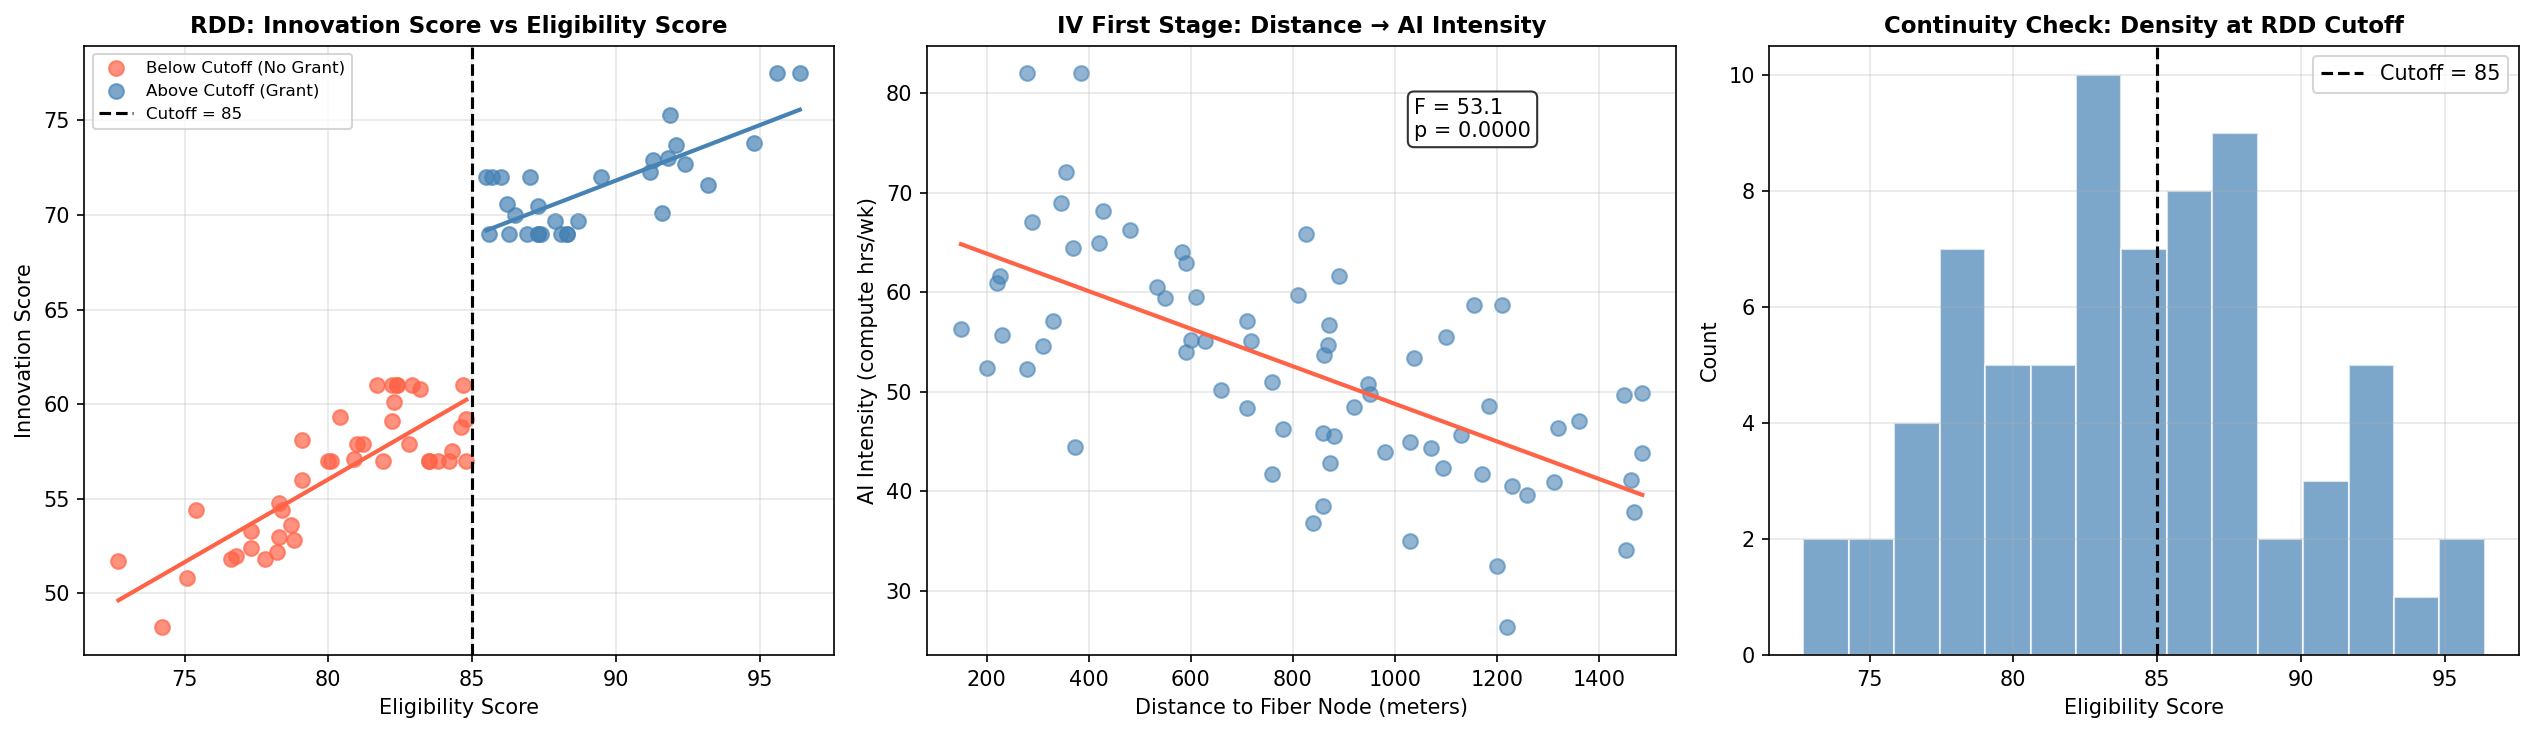
\includegraphics[width=\textwidth]{iv_rdd_plots.png}
    \caption{Left: RDD scatter plot of innovation score vs
    eligibility score with separate regression lines above
    and below the 85-point cutoff, showing a visible upward
    jump. Center: IV first-stage relationship between distance
    to fiber node and AI intensity (F = 53.11). Right: Density
    of eligibility scores showing no bunching at the cutoff,
    supporting the continuity assumption.}
    \label{fig:plots}
\end{figure}

\begin{table}[H]
    \centering
    \caption{Model Comparison: Naive OLS vs IV 2SLS vs RDD}
    \begin{tabular}{lrrrr}
        \toprule
        \textbf{Model} & \textbf{Coefficient} & \textbf{Std. Error} &
        \textbf{p-value} & \textbf{Interpretation} \\
        \midrule
        Naive OLS  & $+0.3245$ & 0.083 & $<$0.001 & Biased upward \\
        IV (2SLS)  & $+0.1119$ & 0.133 & 0.403    & Causal estimate \\
        RDD Jump   & $+8.4873$ & 1.642 & $<$0.001 & At cutoff only \\
        \bottomrule
    \end{tabular}
    \label{tab:models}
\end{table}

\begin{table}[H]
    \centering
    \caption{IV First Stage: AI Intensity on Distance to Fiber Node}
    \begin{tabular}{lrrrr}
        \toprule
        \textbf{Variable} & \textbf{Coefficient} & \textbf{Std. Error} &
        \textbf{t-stat} & \textbf{p-value} \\
        \midrule
        Intercept      & 62.94  & 1.84  & 34.2 & $<$0.001 \\
        DISTANCE\_M    & $-$0.019 & 0.003 & $-$7.3 & $<$0.001 \\
        \midrule
        \multicolumn{5}{l}{F-statistic = 53.11 \quad (Strong instrument: F $>$ 10)} \\
        \multicolumn{5}{l}{$n = 72$ student teams} \\
        \bottomrule
    \end{tabular}
    \label{tab:firststage}
\end{table}

\end{document}
